%-------------------------------------------------------------------------------
% yoshimi-cookbook
%-------------------------------------------------------------------------------
%
% \file        yoshimi-cookbook.tex
% \library     Documents
% \author      Chris Ahlstrom
% \date        2015-07-12
% \update      2016-03-10
% \version     $Revision$
% \license     $XPC_GPL_LICENSE$
%
%     This document provides LaTeX documentation for yoshimi.  It is similar
%     in structure to the yoshimi-doc project.
%
%-------------------------------------------------------------------------------

\documentclass[
 11pt,
 twoside,
 a4paper,
 headinclude,
 footinclude,
 final                                 % versus draft
]{article}

% This file and its clone in yoshimi-doc should be kept in sync:

%-------------------------------------------------------------------------------
% docs-structure
%-------------------------------------------------------------------------------
%
% \file        yoshimi-docs-structure.tex
% \library     Documents
% \author      Chris Ahlstrom
% \date        2015-04-20
% \update      2015-07-14
% \version     $Revision$
% \license     $XPC_GPL_LICENSE$
%
%     This "include file" provides LaTeX options for a document.
%
%     Note that enumitem is an extension of enumerate, and comes from
%     Debian's texlive-latex-recommended package.
%
%-------------------------------------------------------------------------------

\usepackage{enumitem}         % setting the whitespace between and within lists
\setlistdepth{9}
% \setlist{nosep}             % spacing around the list
\setlist{noitemsep}           % spacing within the list

% \usepackage[dvipsnames]{xcolor} % provide more colors?

\usepackage{color}            % provide colors?

% \usepackage[usenames,dvipsnames,svgnames,table]{xcolor}

\usepackage{nameref}          % Provide references by name instead of number
\usepackage[colorlinks=true,linkcolor=webgreen,filecolor=webbrown,citecolor=webgreen]{hyperref}
\definecolor{webgreen}{rgb}{0,.5,0}
\definecolor{webbrown}{rgb}{.6,0,0}

\usepackage{url}              % Required for including URLs
\usepackage{hyperref}         % Required for including hyperlinks
\usepackage{amsthm}           % Helps avoid "destination with same
% \usepackage{cleveref}       % identifier" warnings?
\usepackage[hypcap]{caption}  % make labels point to figure, not the caption
% \usepackage{hypcap}         % make labels point to figure, not the caption
\usepackage[pdftex]{graphicx} % Required for including images
\graphicspath{{../images/}}   % Set the default folder for images
\usepackage{float}            % For more control of location of Figures
\usepackage{geometry}         % Page & text layout
\geometry{
  letterpaper,
  top=2.5cm,
  bottom=2.5cm,
  left=2cm,
  right=2cm
}

\usepackage{longtable}        % For making multi-page tables
\usepackage{makeidx}          % For making an index

% This package isn't available easily on CentOS:
%
% \usepackage[subtle]{savetrees} % For tightening document vertical spacing

\hypersetup{                  % HYPERLINKS
% draft,                      % Uncomment removes links (e.g. for B&W printing)
 colorlinks=true,
 breaklinks=true,
% bookmarks=true,
 bookmarksnumbered,
 urlcolor=webbrown,
 linkcolor=blue,              % RoyalBlue
 citecolor=webgreen,
 pdftitle={},
 pdfauthor={\textcopyright},
 pdfsubject={},
 pdfkeywords={},
 pdfcreator={pdfLaTeX},
 pdfproducer={LaTeX with hyperref and ClassicThesis}
}

% Make an "enumber" style that makes all levels of enumerated lists show
% arabic numerals.

\newlist{enumber}{enumerate}{10}
\setlist[enumber]{nolistsep,label=\arabic*.}

% Make "paragraph" a fourth level, and make it shown in the table of
% contents.

\makeatletter
\renewcommand\paragraph{\@startsection{paragraph}{4}{\z@}%
   {-2.5ex\@plus -1ex \@minus -.25ex}%
   {1.25ex \@plus .25ex}%
   {\normalfont\normalsize\bfseries}}
\makeatother
\setcounter{secnumdepth}{4} % how many sectioning levels to assign numbers to
\setcounter{tocdepth}{4}    % how many sectioning levels to show in ToC

% Provide a way of counting user interface items without putting them in an
% enumberation.

\newcounter{ItemCounter}

% Makes a numbered paragraph out of an item, and allows two index entries
% for it.

\newcommand{\itempar}[2] {
   \stepcounter{ItemCounter}
   \textbf{\arabic{ItemCounter}. #1.}
   \index{#1}
   \index{#2}
}

% Provides for two forms of an option, as might be shown in a man page.

\newcommand{\optionpar}[2] {
   \textbf{\texttt{#1}} \textbf{\texttt{#2}} \\
   \index{#1}
   \index{#2}
}

% Now deprecated in preference to \itempar

\newcommand{\settingdesc}[2] {
   \textbf{#1}
   \index{#1}
   \index{#2}
}

% Make a full reference to a figure using its number, its name, and its page
% number.  Very useful if you have a hard-copy of the document to deal with.

\newcommand{\figureref}[1] {
   figure~\ref{#1}
   ("\nameref{#1}")
   on page~\pageref{#1}\ignorespaces
}

% Make a full reference to a section using its number, its name, and its page
% number.  Very useful if you have a hard-copy of the document to deal with.

\newcommand{\sectionref}[1] {%
   section~\ref{#1}
   ("\nameref{#1}")
   on page~\pageref{#1}\ignorespaces
}

% An attempt to reduce excess vertical space.  Does not work.  See the
% top of yoshimi-user-manual.tex instead.
%
% \setlength{\parindent}{0pt}
% \setlength{\parskip}{0pt}

% Space between floats. \dblfloatsep for 2 column format.
% \setlength{\floatsep}{8pt}

% Space above and below in-line text floats
% \setlength{\intextsep}{8pt}

% Space above float caption
% \setlength{\abovecaptionskip}{8pt}

% Space below float caption
% \setlength{\belowcaptionskip}{8pt}

% Change the fragction of the page that can be filled with graphics from 0.7
% to 0.9.

\renewcommand\floatpagefraction{.9}
\renewcommand\dblfloatpagefraction{.9}
\renewcommand\topfraction{.9}
\renewcommand\dbltopfraction{.9}
\renewcommand\bottomfraction{.9}

%-------------------------------------------------------------------------------
% vim: ts=3 sw=3 et ft=tex
%-------------------------------------------------------------------------------
         % specifies document structure and layout

% Replacing normal header/footer with a fancier version.  These two symbols of
% document class were showing up as "unused" in the log file.
%
% headinclude,
% footinclude,
%
% So we add the fancyhdr package, clear the default layout, and set it up for
% our wider pages.

\usepackage{fancyhdr}
\pagestyle{fancy}
\fancyhead{}
\fancyfoot{}
\fancyheadoffset{0.005\textwidth}
\lhead{Yoshimi Software Synthesizer}
\chead{}
\rhead{Cookbook}
\lfoot{}
\cfoot{\thepage}
\rfoot{}

\makeindex

\begin{document}

\title{A Yoshimi Cookbook}
\author{Chris Ahlstrom\\
   (\texttt{ahlstromcj@gmail.com})}
\date{\today}
\maketitle
\tableofcontents
\listoffigures                         % print the list of figures
\listoftables                          % print the list of tables

% Change the paragraph style to remove indenting and put a line between each
% paragraph.  This could be moved up into the preamble, but then would
% affect the spacing of the TOC and LOF, LOT noted above.

\setlength{\parindent}{0pt}
\setlength{\parskip}{1ex plus 0.5ex minus 0.2ex}

\section{Introduction}
\label{sec:introduction}

   This document is a follow-on to the author's
   "A Yoshimi User Manual" \cite{yoshimidoc}.
   The user manual attempts complete coverage of the user-interface and
   concepts behind \textsl{Yoshimi}.
   This cookbook attempts to provide recipes to solve some common problems
   in getting \textsl{Yoshimi} to perform at its best for the user.

\subsection{Project Structure}
\label{subsec:introduction_project_structure}

   The "Yoshimi Cookbook" project consists of two parts:

   \begin{itemize}
      \item The source material for this document.
      \item A self contained "yoshimi" configuration and data
            section to support the examples in this cookbook.
   \end{itemize}

   The documentation source-files are provided in the \texttt{tex}
   directory.  They are use to create the cookbook via Makefiles and
   the external "latexmk" project.  The result of a "make" is a new
   PDF of the cookbook in the \texttt{pdf} directory.  The latest
   PDF is always provided there so that one does not have to install the
   external projects needed to create it.

   The configuration, banks, presets, and instrument files can be used
   to supplement or replaces the user's own configuration and data files.

\subsection{XML File Compression}
\label{subsec:introduction_xml_files}

   One thing we recommend for following this cookbook is to set the
   \textsl{Yoshimi} compression level to \textbf{0}.  This makes it a lot
   easier to text-edit the file to read its contents.  To make this setting:

   \index{XML compression}
   \begin{enumber}
      \item Navigate to \textbf{Menu / Yoshimi / Settings.../ Main settings}.
      \item Click on the left arrow of \textbf{XML compression level} until
         the value of 0 appears.
      \item Click on the \textbf{Save and Close} button.
      \item Restart \textsl{Yoshimi}, then navigate again to this dialog
         to verify that the setting has been saved.
   \end{enumber}

   Setting this option makes the XML files a bit larger, perhaps larger by a
   factor of more than 10, making a 10K file into a 180K file.
   But these days, that should not be a problem.  Maybe if one is running
   \textsl{Yoshimi} on an old \textsl{Raspberry Pi} device.

\subsection{What Game Shall We Play Today?}
\label{subsec:introduction_what_game}

   There are a number of recipes that are hinted at in the user manual, but
   that solve problems that the author has encountered while using
   \textsl{Yoshimi}.

   \begin{itemize}
      \item \textbf{Banks and MIDI}.
         \textsl{Yoshimi} has had recent modifications to support
         bank-switching and using program-change messages to make
         \textsl{Yoshimi} a more flexible MIDI playback tool.
      \item \textbf{General MIDI}.
         It should be possible to set up one or more banks that
         are General MIDI compliant.
      \item \textbf{Usage of Modulators}.
         \textsl{Yoshimi} provides a number of modulation setups,
         but it isn't clear how to use them, especially the ring modulator.
      \item \textbf{Creation of Special Instruments}.
         There are some instruments that don't seem to have
         decent \textsl{ZynAddSubFX}/\textsl{Yoshimi} instrument files.
         Some examples, based on our desires: sitar, koto, bagpipes, steel
         drums, telephone tones, middle-eastern pipes, Japanese instruments,
         that steel-whip percussion sound heard in many songs....
      \item \textbf{More!}.
   \end{itemize}

   This document explains how to do some of the above tasks.

%  Oh, before you get started, go to
%  \textsl{Menu / Instruments / Open Instruments...} and
%  navigate to where you installed this project (for example,
%  \texttt{~/3rdparty/yoshimi-cookbook/yoshimi/banks} and click
%  \textbf{Add to Favorites} in the \textbf{Favorites} dropdown.
%  That's where we store our GM bank and the demonstration files.

\rhead{\rightmark}         % shows section number and section name

% Concepts

%-------------------------------------------------------------------------------
% cookbook_concepts
%-------------------------------------------------------------------------------
%
% \file        cookbook_concepts.tex
% \library     Documents
% \author      Chris Ahlstrom
% \date        2015-07-15
% \update      2015-07-16
% \version     $Revision$
% \license     $XPC_GPL_LICENSE$
%
%     Provides the concepts.
%
%-------------------------------------------------------------------------------

\section{Concepts}
\label{sec:concepts}

   This section, like its counterpart in our \textsl{Yoshimi User Manual},
   presents some useful concepts, while keeping them out of the way.

\subsection{Concepts / Terms}
\label{subsec:concepts_terms}

   This section doesn't provide comprehensive coverage of terms.  It
   covers mainly terms that puzzled the author at first or that are
   necessary to understand the recipes.

\subsubsection{Concepts / Terms / cent}
\label{subsubsec:concepts_terms_cent}

   The \textbf{cent}
   \index{cent}
   is a logarithmic unit of measure used for musical
   intervals.  Twelve-tone equal temperament divides the octave into 12
   semitones of 100 cents each. Typically, cents are used to measure
   extremely small finite intervals, or to compare the sizes of comparable
   intervals in different tuning systems.
   The interval of one cent is much too small to be heard between
   successive notes.

   Since the detuning provided in \textsl{Yoshimi} is based primarily on
   cents (and octaves), it pays to understand cents.  If a given frequency
   \texttt{f'} is offset from another frequency \texttt{f}, the
   relationships between them in semitones are:

   \[f' = f * 2^s/12\]

   \[s = 12 log (f'/f) / log 2\]

   In cents, these relationships become:

   \[f' = f * 2^s/1200\]

   \[s = 1200 log (f'/f) / log 2\]

   These relationships hold whether \texttt{f'} is less than or greater than
   \texttt{f}.  They provide an easy way to determine how much to detune a
   frequency in \textsl{Yoshimi}.

\subsubsection{Concepts / Terms / ring modulation}
\label{subsubsec:concepts_terms_ring_mod}

   \textbf{Ring modulation}
   \index{ring modulation}
   \index{modulation!ring}
   is the multiplication (heterodyning) of two signals, and is named for the
   ring-like circuit that can produce it.
   When two tones, \texttt{f1} and \texttt{f2}, with 
   \texttt{f1} \textless \texttt{f2}, are multiplied, the spectrum
   changes from \{f1, f2\} to \{f2-f1, f2+f1\}.

   Depending on the ratio of \texttt{f1} and \texttt{f2}, the
   sounds can be bell-like or very discordant.
   \textsl{Yoshimi} provides ring modulation, as well as other forms of
   modulation.

%-------------------------------------------------------------------------------
% vim: ts=3 sw=3 et ft=tex
%-------------------------------------------------------------------------------


% Presets

%-------------------------------------------------------------------------------
% cookbook_presets
%-------------------------------------------------------------------------------
%
% \file        cookbook_presets.tex
% \library     Documents
% \author      Chris Ahlstrom
% \date        2016-03-09
% \update      2016-03-10
% \version     $Revision$
% \license     $XPC_GPL_LICENSE$
%
%     Provides a tutorial on presets.
%
%-------------------------------------------------------------------------------

\section{Fun With Presets}
\label{sec:presets}

   This section expands on its counterpart in the  \textsl{Yoshimi User Manual},
   showing how presets can be employed to re-use blocks of settings.
   In this short tutorial, we will grab and save a number of presets,
   and then use them to partly reconstitute the sound.

\subsection{Presets / Paths}
\label{subsec:presets_paths}

   First, one needs to make sure to have one's
   \texttt{\textasciitilde/.config/yoshimi/presets} directory
   in the set of preset directories.
   Navigate to the \textbf{Main window / Paths / Preset Dirs...} menu entry
   and see if it is there.
   Add it if necessary.

   Second, make sure that there are some root directories available.
   Navigate to the \textbf{Main window / Paths / Bank Root Dirs...} menu entry
   and make sure at least the first of these directories are present:

   \begin{verbatim}
      /usr/share/yoshimi/banks (or in /usr/local if built from source)
      /usr/share/zynaddsubfx/banks
   \end{verbatim}

\subsection{Presets / Pick a Patch}
\label{subsec:presets_pick_a_patch}

   Now navigate to
   \textbf{Main window / Patch Sets / Show Patch Banks...}.
   Pick item \textbf{60. Pads}.
   In the Pads bank window that opens, pick \textbf{8. Resonance Pad1}.
   The following figure shows the set of windows that are now open:

\begin{figure}[H]
   \centering 
   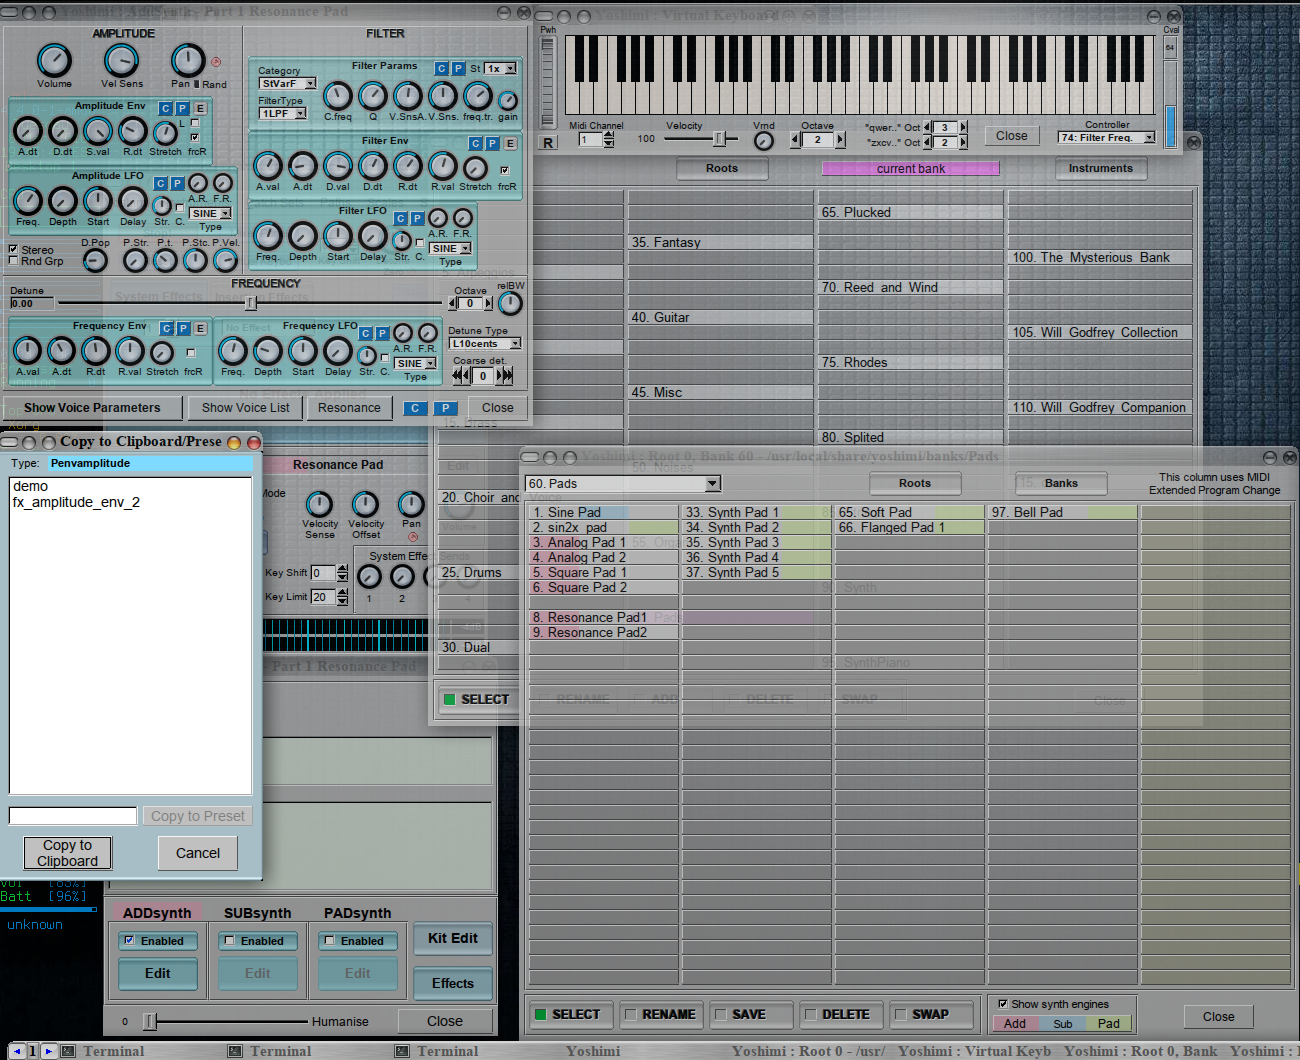
\includegraphics[scale=0.5]{navigating-to-a-preset.png}
   \caption{Navigating to a Preset}
   \label{fig:presets_navigating_to_a_preset}
\end{figure}

   Take a moment to note each of the windows that are open now.
   Play the virtual keyboard for awhile, until the sound of this
   patch/instrument is memorized (we want to reconstruct this sound later).

   Now let's save some of the instrument's presets.
   Click the \textsl{Yoshimi} main window's \textbf{Edit} button.
   Oddly, this PAD instrument uses only the ADDsynth engine.
   Press the ADDsynth item's \textbf{Edit} button.
   Up comes the complex, multi-panelled window for the ADDsynth setup.
   Note the blue \textbf{C} and \textbf{P} buttons in each of the following
   sub-panels:

   \begin{itemize}
      \item \textbf{Amplitude Env}
      \item \textbf{Amplitude LFO}
      \item \textbf{Filter Params}
      \item \textbf{Filter Env}
      \item \textbf{Filter LFO}
      \item \textbf{Frequency Env}
      \item \textbf{Frequency LFO}
      \item The whole \textbf{ADDsynth Window}
   \end{itemize}

   Let's save them all!  Click on each \textbf{C} button,
   then fill in the \textbf{Copy to Preset} text field with
   the name \textsl{"demo"}, and then press the \textbf{Copy to Preset}
   button.  All of the file-names that result will start with
   \texttt{demo}.

   Then click on the \textbf{Show Voice Parameters} button,
   then click on the \textbf{C} button to save the one enabled sub-panel
   for that instrument's voice, \textbf{Frequency LFO}.
   Note that the \textsl{demo} is already saved in this preset of
   type \textsl{Plfofrequency}.  So, if we want to save this, we'd use a
   name other than \textsl{demo}.  Click \textbf{Cancel}.

   Now click on the \textbf{C} button
   for the whole ADDsynth voice window.  Go ahead and do
   \textbf{Copy to Preset} named "demo".

   Now look in \texttt{\textasciitilde/.config/yoshimi/presets}",
   and see all the saved files:
   \index{files!demo.ADnoteParameters.xpz}

\begin{verbatim}
	$ ls ~/.config/yoshimi/presets
	demo.ADnoteParametersn.xpz (whole ADDsynth preset?)
	demo.ADnoteParameters.xpz (whole ADDsynth Voice preset?)
	demo.Penvamplitude.xpz
	demo.Penvfilter.xpz
	demo.Penvfrequency.xpz
	demo.Pfilter.xpz
	demo.Plfoamplitude.xpz
	demo.Plfofilter.xpz
	demo.Plfofrequency.xpz
\end{verbatim}

	Two of them are confounded with the same type, but slightly
   different file-names.  How?

   Now all of these presets are available for loading.
   Let's use them to take a basic sine wave, and build up its settings until
   we have something approximating the \textbf{8. Resonance Pad1} sound.
   Let's try to reconstruct the sound.
   
   Load the \textsl{Yoshimi} \textbf{Simple Sound}. 
   This sound currently cannot be obtained via \textbf{Instruments / Clear}!
   (Bug?)
   Therefore just move to the next part number in the main window.
   Or restart \textsl{Yoshimi}.
   Listen to \textbf{Simple Sound} via the virtual keyboard, and note
   how pure and tone-like it is.
   Then click the main window \textbf{Edit} button, then the
   ADDsynth \textbf{Edit} button.
   Now load all of the presets above by clicking on each \textbf{P}
   button and then selecting the \texttt{demo} entry, 
   as shown in the screen-shot (which shows the Penvamplitude preset).

\begin{figure}[H]
   \centering 
   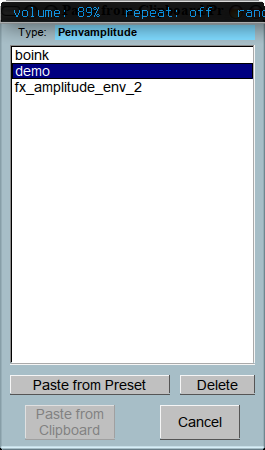
\includegraphics[scale=0.75]{presets/penvamplitude-presets.png}
   \caption{The Penvamplitude Preset}
   \label{fig:presets_penvamplitude}
\end{figure}

   Then click the \textbf{Paste from Preset} button.
   After all this is done, the
   \textbf{Resonance Pad1} sound should 
   be pretty much recovered.
   Pasting the ADDsynth overall preset seems to have the most effect.
   One must play a lot with the presets to fully understand how they work.

   In summary, the presets are essentially keyed to the sub-panels.
   In naming them, you need to use a name that represents the sound that the
   preset contributes, via the settings in its sub-panels.

%-------------------------------------------------------------------------------
% vim: ts=3 sw=3 et ft=tex
%-------------------------------------------------------------------------------


% Instruments

%-------------------------------------------------------------------------------
% cookbook_instruments
%-------------------------------------------------------------------------------
%
% \file        cookbook_instruments.tex
% \library     Documents
% \author      Chris Ahlstrom
% \date        2015-07-12
% \update      2015-07-18
% \version     $Revision$
% \license     $XPC_GPL_LICENSE$
%
%     Provides the cookbooks_instruments section of yoshimi-cookbook.tex.
%
%-------------------------------------------------------------------------------

\section{Creating Instruments}
\label{sec:cookbook_instruments}

   One of our goals in using \textsl{Yoshimi} is to support
   \textsl{General MIDI} (\textsl{GM})
   to the greatest extent possible.

   However, no banks have been created with GM in mind.  And many of the
   instruments, though given names that indicate what they are intended to
   be, fall well short of being recognizable per their name; they should be
   doable with a complex synthesizer like \textsl{Yoshimi}.
  
   It is true that there are a vast number of \textsl{Yoshimi} and
   \textbf{ZynAddSubFX} patches/parts/instruments out there.  The author
   had attempted a survey of them, and the task was all but impossible.
   Still, many candidates have been identified.  Other candidates might be
   suitable with a little tweaking.

   Here are a number of categories of instruments for which we want to
   assemble an improved set of instruments.

   \begin{enumber}
      \item \textbf{Bells}
      \item \textbf{Ethnic}
      \item \textbf{Drums}
      \item \textbf{Effects}
      \item \textbf{Piano}
      \item \textbf{Leads}
      \item \textbf{Guitar}
      \item \textbf{Strings} (individual and ensemble)
      \item \textbf{Bass}
      \item \textbf{Saxophones}
   \end{enumber}

   For these recipes, the \texttt{banks} directories will
   be stored in the following directory of this project:
   \index{directories!demo bank}

   \begin{verbatim}
      yoshimi/banks
      yoshimi/banks/demo
   \end{verbatim}

\subsection{Bells}
\label{subsec:cookbook_instruments_bells}

   The bells patches we've heard so far are nice, but a bit anemic.
   
   \index{ring modulation}
   Good bell patches are easier with ring modulation, done right.  We're not
   sure if there are any such patches extant; please send us to them if
   there are some.

   \index{bells}
   In the meantime, creating bells is a good excuse to master
   \textsl{Yoshimi}'s ring modulator.
   However, we will first learn how to create a reasonable, clangy bell
   using just a few voices in an ADDsynth part, and no need for modulation.

\subsubsection{Bells by Voices}
\label{subsec:cookbook_instruments_bells_by_voices}

   The following table comes from a tutorial (\cite{bellsimple}).  Along
   with a spectrum shown in reference \cite{bellspectrum}, it allows us to
   recreate a simple, but realistic bell.
   \index{bells!spectrum}
   In this table, \texttt{F} represents the fundamental frequency, i.e. the
   note being played.

\label{table:simple_bell_tones}
\begin{longtable}{c c c c}
   \caption{Simple Bell Tones} \\
   \hline
      \textbf{Wave Number} &
      \textbf{Frequency} &
      \textbf{Cents Offset} &
      \textbf{Relative Amplitude} \\
   \hline
   \endfirsthead

   1 &  0.56F &  -1000 &   0.5   \\
   2 &  0.92F &  -140  &   1.0   \\
   3 &  1.19F &  +300  &   0.5   \\
   4 &  1.71F &  +930  &   0.25  \\
   5 &  2.00F &  +1200 &   0.125 \\
   6 &  2.74F &  +1745 &   0.125 \\
   7 &  3.00F &  +1901 &   0.125 \\
   8 &  3.76F &  +2290 &   0.125 \\
   9 &  4.00F &  +2400 &         \\
\end{longtable}

   Note that the frequencies are relative to the fundamental frequency (F).
   Also note that wave 2 (close to F) can be missing, and the sound still is
   bell-like.

   \index{files!bells addsynth}
   The file \texttt{yoshimi/banks/demo/Bells-simple-addsynth.xiz} is the
   result of following the steps below.  We start, as usual, with a
   newly-started \textsl{Yoshimi} instance.

   \begin{enumber}
      \item Open the ADDsynth editing window by clicking the \textbf{Edit}
         button in the bottom panel, and then clicking the ADDsynth
         \textbf{Edit} button in the edit window.
      \item Click on the \textbf{Show Voice Parameters} button.
         Note that it is \textbf{Current Voice 1}, and it should be enabled.
      \item For voice 1, make the following settings:
         \begin{enumber}
            \item \textbf{Octave}: Set to 0.
            \item \textbf{Detune Type}: Set to E1200cents.
            \item \textbf{FREQUENCY Detune}: Set to -1000 approximately.
         \end{enumber}
      \item Go to voice 2, and make the following settings:
         \begin{enumber}
            \item \textbf{Octave}: Set to 0.
            \item \textbf{Detune Type}: Set to E1200cents.
            \item \textbf{FREQUENCY Detune}: Set to -140 approximately.
         \end{enumber}
      \item Go to voice 3, and make the following settings:
         \begin{enumber}
            \item \textbf{Octave}: Set to 0.
            \item \textbf{Detune Type}: Set to E1200cents.
            \item \textbf{FREQUENCY Detune}: Set to 300 approximately.
         \end{enumber}
      \item Go to voice 4, and make the following settings:
         \begin{enumber}
            \item \textbf{Octave}: Set to 0.
            \item \textbf{Detune Type}: Set to E1200cents.
            \item \textbf{FREQUENCY Detune}: Set to 930 approximately.
         \end{enumber}
      \item Go to voice 5, and make the following settings:
         \begin{enumber}
            \item \textbf{Octave}: Set to 1.
            \item \textbf{Detune Type}: Set to Default.
            \item \textbf{FREQUENCY Detune}: Set to 0.
         \end{enumber}
      \item Go to voice 6, and make the following settings:
         \begin{enumber}
            \item \textbf{Octave}: Set to 1.
            \item \textbf{Detune Type}: Set to E1200cents.
            \item \textbf{FREQUENCY Detune}: Set to 545 approximately.
         \end{enumber}
      \item Go to voice 7, and make the following settings:
         \begin{enumber}
            \item \textbf{Octave}: Set to 1.
            \item \textbf{Detune Type}: Set to E1200cents.
            \item \textbf{FREQUENCY Detune}: Set to 700 approximately.
         \end{enumber}
      \item Go to voice 8, and make the following settings:
         \begin{enumber}
            \item \textbf{Octave}: Set to 1.
            \item \textbf{Detune Type}: Set to E1200cents.
            \item \textbf{FREQUENCY Detune}: Set to 1090 approximately.
         \end{enumber}
   \end{enumber}

   These settings then end up roughly matching the settings of the first 8
   waves in \tableref{table:simple_bell_tones}.
   \index{bells}
   This instrument isn't perfect.  It's not quite equally tempered, though
   close.  The character of the tone changes a bit as the notes get higher.
   One can fiddle with the relative amplitudes of the various voices to
   change the character of this sound.

\subsubsection{Ring Modulation with 440 Hz Tone}
\label{subsec:cookbook_instruments_ring_mod_440}

   Now for an initial demonstration of ring modulation.
   This demonstration does not quite create a bell tone, but does show
   the sound of modulation.

   Start with a fresh \textsl{Yoshimi} and a cleared instrument ("Simple
   Sound").  Open the virtual keyboard using the \textbf{virKbd} button.
   Click a key and verify that you can hear a tone.
   \index{"C" note}
   \index{comma key}
   We'll use the middle C
   key (the "comma" on the PC keyboard) as a reference.  We will call it
   the "C" note.

   The following steps will set up two tones, voice 1 and voice 2, and voice
   2 will use voice 1 as an external modulator.
   Note that you can accomplish most of these steps by loading the project
   file
   \index{bells}
   \index{files!bells 440}
   \texttt{yoshimi/banks/demo/Bells-440-ring-modulation.xiz}, but use
   that only as a last resort.

   \begin{enumber}
      \item Open the ADDsynth editing window by clicking the \textbf{Edit} button
         in the bottom panel, and then clicking the ADDsynth \textbf{Edit}
         button in the edit window.
      \item In the \textbf{Amplitude Env} sub-panel, increase the
         \textbf{D.dt} and \textbf{R.dt} to give the current
         sound a nice slow decay.
      \item Click on the \textbf{Show Voice Parameters} button.
         Note that it is \textbf{Current Voice 1}, and it should be enabled.
      \item Switch to \textbf{Current Voice} number 2 and enable it.
         Play the "C" note, and observe that it is the same frequency, but
         louder.
      \item Move the \textbf{FREQUENCY Detune} slider a bit, and play the "C"
         note.  It should sound the same as before, but change slowly in
         amplitude, as heard and as seen on the \textbf{VU meter}.
         Try to set the detune back to 0; this is easier if you highlight
         the tuning knob and use the left or right arrow keys.
      \item In the \textbf{MODULATOR} section of voice 2, for \textbf{Type},
         select the \textbf{RING} value.  (However, feel free to select one
         of the other modulators, to experiment, once you've mastered
         the ring modulator.)  Press the "C" key again, and notice
         that the tone character changes a bit.  This is due to the internal
         modulator.
      \item For \textbf{External Mod.} for voice 2, select
         \textbf{Ext.M} 1, to use the voice 1 as the internal modulator.
         The "C" note may change in character, but only slightly.
         Apparently the default internal modulator is the same as the
         default external voice 1 waveform.
      \item To actually hear some modulation, we have to separate the
         frequencies of voice 1 and voice 2.  Click the \textbf{440Hz}
         check-box in the \textbf{FREQUENCY} section of voice 1.  Press the
         "C" key and verify hearing a two-tone signal, somewhat like a phone
         tone.
      \item Now go back to voice 2 and click the \textbf{Change} button to
         bring up the ADDsynth oscillator dialog.
      \item Move the slider to maximum for harmonic 10.  Press the "C" key
         and verify the new sound (a bit like a car horn).
         Set the sliders back to 0, and "C" will be a single tone again.
      \item Change the \textbf{Octave} values of voice 2 in its
         \textbf{FREQUENCY} section and listen to the effects.
   \end{enumber}

   Now we need to see if we can apply modulation across instruments.
   Sadly, this does not seem to be possible.

   Increase the \textbf{D.dt} and \textbf{R.dt} values of the main
   \textbf{Amplitude Env} to give this sound the onset and decay of a bell,
   and it then sounds less abstract, and more like a bell.
   Of course, this kind of bell is even less tunable than the simple
   bell of the previous section.

   Another thing to try with this setup is to simply change voice 2 to use
   different types of modulators besides \textbf{RING}.
   \textbf{MORPH} sounds basically identical to \textbf{RING}.
   \textbf{PM} seems to expose higher harmonics, making the sound louder and
   brighter.
   \textbf{FM} sounds similar to PM, but softer and smoother.
   \textbf{PITCH} is disabled.

   Another experiment is to disable the modulator (voice 1 here) and see how
   that changes the sound; all it should do is drop voice 1 from the
   spectrum -- voice 1 will still be used as the modulator.

   Finally, by adding a slow decay to this sound, it becomes amazingly more
   bell-like.

\subsubsection{Complex Bells by Ring Modulation}
\label{subsec:cookbook_instruments_bells_by_ring_mod}

   The next step is to make the bells more complex, by combining the methods
   of the previous two sections.
   Recall \tableref{table:simple_bell_tones}.
   It shows the 9 frequencies in the simple bell spectrum, though we could
   define only 8 of them.  How can we best add extra frequencies?
   \index{bells}
   We can ring-modulate the higher frequencies against one of the lower
   frequencies.

\label{table:ring_mod_bell_tones}
\begin{longtable}{l l l l l}
   \caption{Ring Modulation Bell Tones} \\
   \hline
      \textbf{Wave Number} &
      \textbf{Frequency} &
      \textbf{Mod Frequency} &
      \textbf{f2-f1} &
      \textbf{f2+f1} \\
   \hline
   \endfirsthead

   1 &  0.56F &  ----- &  -----   &  -----   \\
   2 &  0.92F &  0.56F &  0.36F   &  1.48F   \\
   3 &  1.19F &  0.56F &  0.63F*  &  1.75F*  \\
   4 &  1.71F &  0.56F &  1.15F*  &  2.27F   \\
   5 &  2.00F &  0.56F &  1.44F   &  2.56F   \\
   6 &  2.74F &  0.56F &  2.18F   &  3.30F   \\
   7 &  3.00F &  0.56F &  2.44F   &  3.56F   \\
   8 &  3.76F &  0.56F &  3.20F   &  4.32F   \\
\end{longtable}

   The asterisk marks frequencies that are close to existing
   frequencies.   Luckily, there are only three of them, so our
   modulation should add a good number of frequencies.

   \index{files!bells addsynth}
   \begin{enumber}
      \item Load the file \texttt{yoshimi/banks/demo/Bells-simple-addsynth.xiz}
         to save a lot of steps.  The next steps add voice 1 as a ring
         modulator for voices 2 through 8.
      \item Open the ADDsynth editing window by clicking the \textbf{Edit}
         button in the bottom panel, and then clicking the ADDsynth
         \textbf{Edit} button in the edit window.
      \item Click on the \textbf{Show Voice Parameters} button.
         Note that it is \textbf{Current Voice 1}, and it should be enabled.
      \item Go to voice 2 and do the following steps:
         \begin{enumber}
            \item In the \textbf{MODULATOR} section (greyed out), change the
               \textbf{Type} from \textbf{OFF} to \textbf{RING}.
            \item Changes the \textbf{External Mod.} dropdown from
               \textbf{Off} to \textbf{ExtMod. 1}.
         \end{enumber}
      \item Go to voice 3 and repeat those steps.  Note how all the voices
         below the current voice become available as modulators.
   \end{enumber}

   We saved the result in the file
   \index{files!bells ring mod}
   \texttt{yoshimi/banks/demo/Bells-ringmod-addsynth.xiz} for safe-keeping.

   QUESTION:  If one loads and instrument and tinkers with it, but do not
   save it, does \textsl{Yoshimi} save it on exit anyway?

\subsection{Ethnic}
\label{subsec:cookbook_instruments_ethnic}

   We've found a simple steel drum instruments, but think we might do better,
   creating one using ADDsynth and one using PADsynth.

   Instruments we have not found, and would like to synthesize, are:
   bagpipes and arabic pipes.

\subsubsection{Ethnic / Steel Drums}
\label{subsubsec:cookbook_instruments_ethnic_steeldrums}

   \index{steel drums}
   There is a steel-drum instrument that ships with \textsl{Yoshimi}:
   \index{files!steel drums}
   \texttt{/usr/share/yoshimi/banks/The\_Mysterious\_Bank/0122-pseudo\_steeldrums.xiz}.
   It is an ADDsynth module comprised of three voices:

   \begin{enumber}
      \item A \textbf{Unison}-enabled voice of \textbf{Size} = 10 and a
         \textbf{Frequency Spread} of 44.6 cents.
      \item Another voice that is exactly the same as the first, except that
         it has its \textbf{Amplitude Env} sub-panel enabled, to add more
         volume and character to the instrument, it is stronger on the
         right, and, most importantly, an octave higher.
      \item Another voice that is exactly the same as the second, 
         except it is an octave lower than voice 0.
   \end{enumber}

   If voice 2 and 3 are disabled, the instrument still sounds reminiscent of
   steel drums, so obviously the overall amplitude envelope is important.

   Can we do better?  Well, the instrument above sounds too pristine.
   We should be able to add some "dirt" to the instrument to make it sound
   more lively.

\begin{figure}[H]
   \centering 
   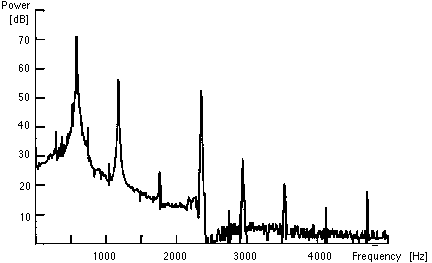
\includegraphics[scale=0.85]{contrib/steel_drum_spectrum.png}
   \caption{Typical Steel Drum Spectrum}
   \label{fig:cookbook_bank_steeldrum_spectrum}
\end{figure}

   Taking a cue from this figure, our steel drums extend the original
   by adding a couple more tones at octave intervals.  Also, some slight
   detuning was introduced to add to the flavor.
   We could probably add a couple more, and carefully contour their
   amplitude levels to match the spectrum levels shown above.

   To hear the ADDsynth steel drum sound, load the file
   \index{files!steel drums}
   \texttt{yoshimi/banks/demo/Add\_Pseudo\_Steel\_Drums.xiz}.

   Not content with that, with our hands behind our back, we pull
   SUBsynth from a hat.  The SUBsynth settings for a steel drum are shown in
   the following figure:

\begin{figure}[H]
   \centering 
   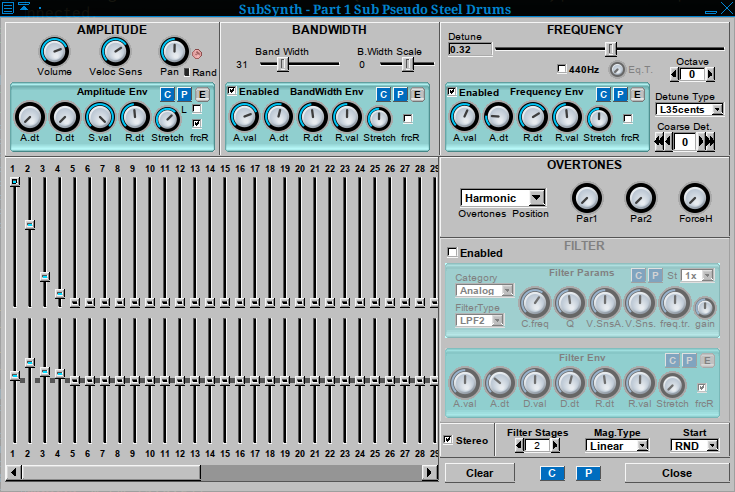
\includegraphics[scale=0.75]{demo/steeldrums-subsynth-editor.png}
   \caption{Steel Drum SUBsynth Configuration}
   \label{fig:cookbook_bank_steeldrum_subsynth}
\end{figure}

   Note the top box of slider controls.  It sets the amplitudes of
   the harmonics, and should vaguely resemble the spectrum diagram.
   The lower box of slider controls sets the bandwidth of each harmonic,
   with the fundamental frequency being very narrow.

   To hear the SUBsynth steel drum sound, load the file
   \index{files!steel drums}
   \texttt{yoshimi/banks/demo/Sub\_Pseudo\_Steel\_Drums.xiz}.
   It's pretty nasty.

   However, the best steel drum patch we've encountered so far is the
   \texttt{banks/olivers-100/0029-Steel Drums.xiz} from the installed banks
   of \textsl{ZynAddSubFx}, and that's the one we now copy to
   our cookbook project's 
   \texttt{yoshimi/banks/gm-basic/0115-Steel Drums.xiz} GM slot.

\subsection{Drums}
\label{subsec:cookbook_instruments_drums}

   We want a decent drum kit that attempts to fill in the gaps for a
   GM-compliant drum kit with solid sounds, with
   the help of an existing kit.

   It turns out that a "Natural Drum Kit", which we'd found separately on
   the Internet (from Dario Straulino) a long time ago, is now part of the
   instruments installed with \textsl{Yoshimi}.
   \index{drum kit}
   \index{GM!drum kit}
   But long ago we used some of the sounds
   from various kits to create our own "natural drum kit", and extended some
   of the sounds across more (pitched) keys so that any MIDI drum note would
   produce \textsl{some} sound.  We also made sure the sounds were laid out
   in GM format as much as possible.

   Fire up \textsl{Yoshimi} and load the instrument stored in
   \index{files!natural drums}
   \texttt{yoshimi/banks/demo/Natural\_Drum\_Kit\_Basic.xiz}, and we'll walk
   through it.  Click the \textbf{Edit} button in the bottom panel, and then
   click the \textbf{Kit Edit} button.

\begin{figure}[H]
   \centering 
   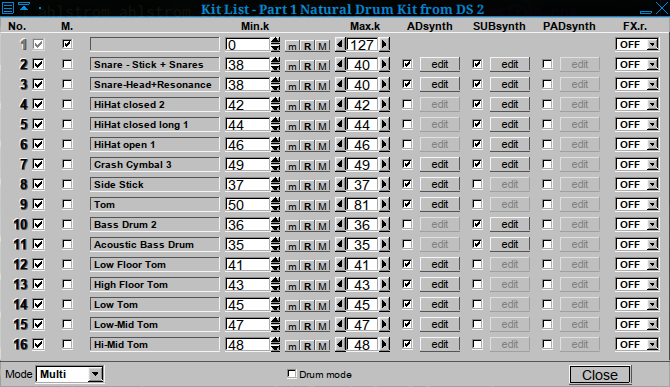
\includegraphics[scale=0.85]{demo/natural_drum_kit_from_ds_2.png}
   \caption{Natural Drum Kit from DS 2}
   \label{fig:cookbook_bank_natural_drum_kit}
\end{figure}

   \textbf{Item 1} is the master control for the whole kit, determining the
   range of keys that it covers and the effect (if any) it goes through.

   \textbf{Item 2} and \textbf{Item 3} provide the two parts of the
   "natural" snare drum.  Both parts are composed of an ADDsynth and a
   SUBsynth section, and they provide 3 pitches of snare.

   \index{natural drum!snare}
   One distinguishing feature of the "Snare - Stick + Snares" item
   is it's only ADDsynth voice.  Clickthe ADDsynth \textbf{Edit} button for
   item 2 in the kit editor.  Then Click on the
   \textbf{Show Voice Parameters} button.
   Note that the \textbf{Amplitude Env} sub-panel is enabled, and uses a
   Freemode envelope.  The voice is locked on \textbf{440Hz}, but detuned to
   be a lot lower than that.  The \textbf{Voice Oscillator}
   (click on the \textbf{Change} button) uses a
   \index{power function}
   \textbf{Base F.} (function)
   set to \textbf{Power}
   \index{pulse}
   to generate a spike pulse.
   There doesn't seem to be a way to temporarily mute an item, so we cannot
   hear what this item would sound like on its own.

   The SUBsynth part of the "Snare - Stick + Snares" item provide an
   \textbf{Amplitude Env}, \textbf{Bandwidth Envelope}, and a rich set of
   alternate harmonics of very narrow bandwidth.

   The "Snare-Head+Resonance" item's ADDsynth settings 
   provide Freemode \textbf{Amplitude Env} and \textbf{Frequency Envelope}
   settings with the voice locked on \textbf{440Hz}, but detuned to
   be a lot lower than that.  The \textbf{Voice Oscillator} is a sine wave.
   Voice 2 is set to \textbf{NOISE}, but is disabled.  Something to try out?
   Indeed, we changed voice 2 to a sine wave, moved it up an octave,
   and now the the Snare keys have slightly different qualities, a barely
   noticeable pitch.  A keeper!

   The "Snare-Head+Resonance" item's SUBsynth settings are a set of
   harmonics with a \textbf{Bandwidth Env}.

   \index{natural drum!hihats}
   \textbf{Item 4} is the "HiHat closed 2" instrument, a SUBsynth-only item.
   It provides an \textbf{Amplitude Env}, a \textbf{Bandwidth Env},
   and a \textbf{Frequency Env} centered around 440 Hz, offset downward 2
   octaves.  A number of harmonics are provided, obviously taken from some
   spectral diagram of a cymbal.

   \textbf{Item 5} is the "HiHat closed long 1" instrument, a SUBsynth-only
   item.  It is the same as the "HiHat closed 2" instrument, but with a
   longer amplitude envelope.

   \textbf{Item 6} is the "HiHat open 1" instrument, a SUBsynth-only item.
   Much like the other hi-hats, but with a Freemode
   \textbf{Bandwidth Envelope}.

   \index{natural drum!cymbal}
   \textbf{Item 7} provides the "Crash Cymbal 3" item.
   It is composed of an ADDsynth and a SUBsynth section.
   The ADDsynth provides a \textbf{Voice Oscillator} that, like
   \textbf{Item1}, uses a \index{power function}
   \textbf{Base F.} (function)
   set to \textbf{Power}
   \index{pulse}
   to generate a spike pulse.

   The SUBsynth section is similar to that of the
   "Snare-Head+Resonance" (\textbf{Item 3}), a set of
   harmonics with a \textbf{Bandwidth Env}.

   \index{natural drum!side stick}
   \textbf{Item 8} is the "Side Stick" instrument, an ADDsynth-only item.
   It's only voice, voice 1, is filtered white noise.
   One can increase the \textbf{Q} value of the filter to make it a bit
   metallic.  One can lower the \textbf{C.freq} value to make it sound like
   a bigger stick.

   \index{natural drum!pitched toms}
   \textbf{Item 9} is the "Tom".  It is just a tone with an AR frequency
   envelope.  The puzzling thing is that it is locked to 440 Hz plus 2
   octaves, but it can run the full length of keys 50 to 81 (so we can get
   "Extra toms") and gradually rise in pitch.  How?  Unlocking voice 1 seems
   to change nothing!

   \index{natural drum!bass drums}
   \textbf{Item 10} is "Bass Drum 2", a SUBsynth patch.
   Like the SUBsynth part of the "Snare - Stick + Snares" item, it provides
   a Freemode \textbf{Amplitude Env} and \textbf{Bandwidth Envelope}, but
   only a small set of low harmonics, and a -3 \textbf{Octave} offset, one
   octave lower than the snare.

   \textbf{Item 11} is "Acoustic Bass Drum".  It merely adds some more
   harmonics to the "Bass Drum 2" patch.

   \index{natural drum!toms}
   \textbf{Item 12} is the "Low Floor Tom", an ADDsynth patch.
   Voice 1, like \textbf{Item 9}, is a pitched tone with a frequency
   envelope.  Voice 2 is added to provide a noisy component.

   \textbf{Item 13} through \textbf{16} are also noisy toms.
   At some point, we'll try to use the XML files to determine how their
   pitches are determined.  To difficult to compare the two GUIs without
   taking screen shots.

   Okay, so this drum kit is a little tom-heavy!

   Now, without defining more than one drum kit, we have only about 15
   "drums" available to us in \textsl{Yoshimi}.  So we filled in the missing
   drums with more "toms", just so some sound will be made.  The frequencies
   of the upper toms get pretty crazy!  Here's a diagram of the keyboard
   layout.  Correlate it with
   \figureref{fig:cookbook_bank_natural_drum_kit}, to understand the
   abbreviations.

\begin{figure}[H]
   \centering 
   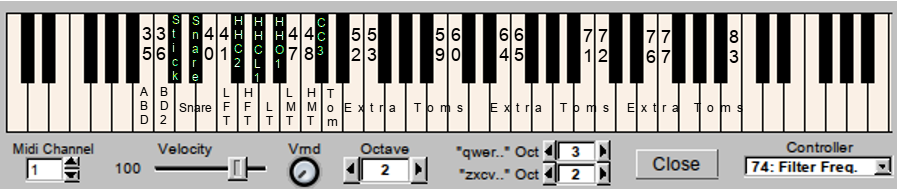
\includegraphics[scale=0.75]{demo/natural_drum_keyboard_layout.png}
   \caption{Natural Drum Kit Keyboard Layout}
   \label{fig:cookbook_bank_natural_drum_kit_layout}
\end{figure}

   For your reference, here is the full GM drum layout.  The diagram is
   taken from WikiMedia.org.

\begin{figure}[H]
   \centering 
   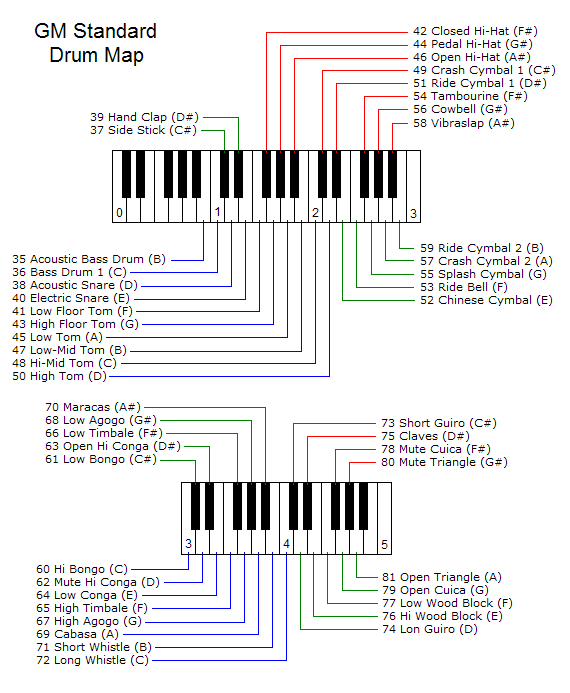
\includegraphics[scale=0.75]{demo/GMStandardDrumMap.png}
   \caption{General MIDI Drum Kit Keyboard Layout}
   \label{fig:cookbook_bank_general_drum_kit_layout}
\end{figure}

\subsection{Chromatic Percussion}
\label{subsec:cookbook_instruments_chromperc}

   One of the big blanks in the gm-basic sound set are the various
   stand-alone percussion instruments:
   woodblock, taiko drum, melodic tom, synth drum, and reverse cymbal.
   These occupy GM slots 116 through 120.

   One easy way to obtain these instruments is to find them in an existing
   drum kit, and extract each into its own instrument file.  Here is how we
   did it to obtain instrument 118, the Melodic Tom.

   First, set up a presets directory to hold any presets one creates, and
   make it the default presets directory.  For example, one can
   set this project's \texttt{yoshimi/presets} directory as the default
   location for preset files.

      \begin{enumber}
         \item Navigate to \textbf{Menu / Settings... / Preset Dirs}
            (a tab in the settings dialog).
         \item Click the \textbf{Add preset directory} button.
         \item Navigate to the desired directory, select it, click
            \textbf{OK}.
         \item Select the new preset directory, then click the
            \textbf{Make default} button.
         \item Press the \textbf{Save and Close} button.
         \item Restart \textsl{Yoshimi}.
      \end{enumber}

   Next, extract the Tom drum from the Natural Drum Kit for use as Melodic
   Tom GM patch:

      \begin{enumber}
         \item Load the "Natural Drum Kit" instrument.
         \item Click \textbf{Edit} to bring up the overall editor dialog.
         \item Then click the \textbf{Kit Edit} button.
         \item Move to item 9, "Tom", and click the
            \textbf{Edit} button to access its ADDsynth settings (the Global
            dialog).
         \item Press the blue \textbf{C} button in the ADDsynth Global
            dialog.
         \item Next to the grayed-out \textbf{Copy to Preset}
            button, give the setting (to be saved) a name:
            "Nat Drum ADDsynth Tom Part".  See the figure below.
         \item Press the now active \textbf{Copy to Preset} button.
         \item Depending on what dialog one is in when pressing the
            \textbf{C} button, the file will be save in the default preset
            \index{files!.ADnoteParameters.xpz}
            directory under a name like \texttt{.ADnoteParameters.xpz}.
      \end{enumber}

\begin{figure}[H]
   \centering 
   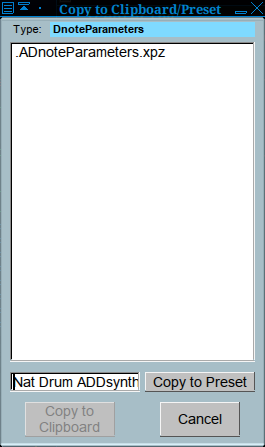
\includegraphics[scale=0.85]{demo/copy_to_clipboard.png}
   \caption{Copy to Clipboard Preset}
   \label{fig:cookbook_instruments_copy_to_clipboard}
\end{figure}

   \index{files!.ADnoteParameters.xpz}
   One should then copy the \textbf{.ADnoteParameters.xpz} file to a file
   with the name \textbf{Nat Drum ADDsynth Tom Part} (matching the name of
   the preset it holds), and restart Yoshimi.
   However, it is only accessible with the hidden file name in the
   \textbf{Paste From Clipboard} dialog, as far as we can tell.

   Finally, the preset can then be loaded into a new instrument as follows:

      \begin{enumber}
         \item Navigate to \textbf{Menu / Instrument / Clear Instrument}, and
            click \textbf{Yes} at the prompt.
         \item Navigate to the desired settings dialog.  In this case, it
            will involve clicking \textbf{Edit}, then the ADDsynth
            \textbf{Edit} button.
         \item In the \textbf{ADDsynth Global} dialog,
            press the blue \textbf{P} button in that dialog,
            to open the \textbf{Paste From Clipboard} dialog.
         \item Select the desired preset (that matches the current settings
            dialog).  In this case, it will be
            \index{files!.ADnoteParameters.xpz}
            \textbf{.ADnoteParameters.xpz}.
         \item Press the \textbf{Paste from Preset} button.
         \item Open the virtual keyboard using the \textbf{virKbd} button,
            and verify that the instrument sounds like the proper Tom kit
            item.
         \item Go back to the Main edit dialog and change the \textbf{Type}
            to the best matching value; here, it would be
            \textbf{Chromatic Percussion}.  Then fill in the
            \textbf{Author and Copyright} and \textbf{Comments} fields.
         \item In the main \textsl{Yoshimi} window, right-click on the part
            name.  In the prompt for \textbf{Instrument name}, type the name
            of the instrument/part; in this case, "Melodic Tom".
         \item Navigate to
            \textbf{Menu / Instrument / Save instrument...}.
            Navigate to the desired directory, append the name (e.g.
            "Melodic Tom.xiz"), and save it.
      \end{enumber}

   It is wise to restart \textsl{Yoshimi} and verify that the new instrument
   can be loaded and played.

\subsection{Effects}
\label{subsec:cookbook_instruments_effects}

   This section documents the various "effects" instruments we've created.

\subsubsection{Effects / Dial Tones}
\label{subsubsec:cookbook_instruments_effects_dialtones}

   \index{effects!dial tone}
   We've created a nice dial-tone effect that we'll describe here.
   Dial tones consist of two notes, as shown by the
   \textbf{Low F} and \textbf{High F} columns in the following table.

\label{table:effect_dial_tones}
\begin{longtable}{l l l l l l l l l l}
   \caption{DTMF Frequencies Table} \\
   \hline
      \textbf{Tag} &
      \textbf{DTMF} &
      \textbf{Kit\#} &
      \textbf{MIDI\#} &
      \textbf{Low} &
      \textbf{Low F} &
      \textbf{Actual F} &
      \textbf{High} &
      \textbf{High F} &
      \textbf{Actual F} \\
   \hline
   \endfirsthead

   1 &  1        & 5  & 53 & F3 &  697 &  705 &  F5     & 1209 &  1245  \\
   2 &  2        & 6  & 77 & F5 &  697 &  705 &  F5     & 1336 &  1337  \\
   3 &  3        & 7  & 89 & F6 &  697 &  698 &  F5     & 1477 &  1468  \\
   4 &  4        & 8  & 55 & G3 &  770 &  770 &  G5 -   & 1209 &  1236  \\
   5 &  5        & 9  & 79 & G5 &  770 &  776 &  G5 -   & 1336 &  1334  \\
   6 &  6        & 10 & 91 & G6 &  770 &  773 &  G5 -   & 1477 &  1462  \\
   7 &  7        & 11 & 57 & A3 &  852 &  855 &  G\#5 + & 1209 &  1245  \\
   8 &  8        & 12 & 81 & A5 &  852 &  868 &  G\#5 + & 1336 &  1327  \\
   9 &  9        & 13 & 93 & A6 &  852 &  866 &  G\#5 + & 1477 &  1480  \\
   * &  *        & 14 & 59 & B3 &  941 &  948 &  A\#5 + & 1209 &  1257  \\
   0 &  0        & 15 & 83 & B5 &  941 &  968 &  A\#5 + & 1336 &  1281  \\
  \# &  \#       & 16 & 95 & B6 &  941 &  950 &  A\#5 + & 1477 &  1480  \\
   A &  A        & -- & -- & A2 &  697 &  --- &  F5     & 1633 &  ---   \\
   B &  B        & -- & -- & B2 &  770 &  --- &  G5 -   & 1633 &  ---   \\
   C &  C        & -- & -- & C2 &  852 &  --- &  G\#5 + & 1633 &  ---   \\
   D &  D        & -- & -- & D2 &  941 &  --- &  A\#5 + & 1633 &  ---   \\
   b &  busy     & 2  & 71 & B4 &  480 &  472 &  B4 -   & 620  &  622   \\
   r &  ringback & 3  & 69 & A4 &  440 &  440 &  A4     & 480  &  480   \\
   d &  dialtone & 4  & 65 & F4 &  350 &  350 &  F4     & 440  &  440   \\
\end{longtable}

   This table is implemented in a \textsl{Yoshimi kit}.  Each note in the
   kit is created by making an ADDsynth instrument with two voices.  The
   lower voice generally corresponds to the note being play, with an offset,
   if needed, to achieve close to the proper frequency for the lower note of
   the DTMF tone.
   The second voice corresponds to the other note, and it is detune
   appropriately to achieve close to the proper frequency for the upper note
   of the DTMF tone.

   The following figure shows the kit dialog:

\begin{figure}[H]
   \centering 
   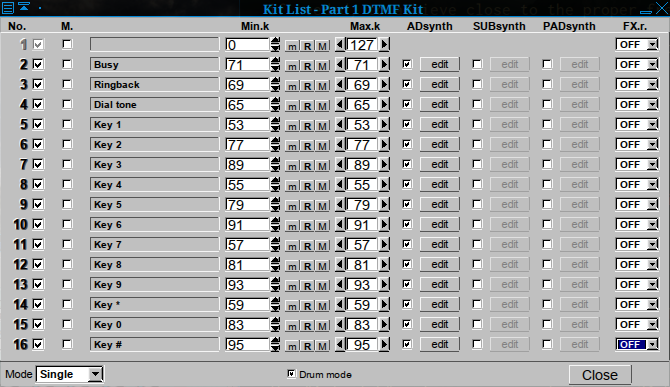
\includegraphics[scale=1.0]{demo/DTMF_kit_edit.png}
   \caption{Kit Edit Dialog for DTMF Kit}
   \label{fig:cookbook_instruments_dtmf_kit_edit}
\end{figure}

   To edit the kit, follow the steps below.  If desired, open the
   instrument file
   \index{files!DTMF kit}
   \texttt{yoshimi/banks/demo/DTMF\_Kit.xiz} to save some
   work.

   \begin{enumber}
      \item Open the kit editing window by clicking the \textbf{Edit}
         button in the bottom panel, and then clicking the
         \textbf{Kit Edit} button in the edit window.
      \item Make sure that the \textbf{Mode} is set to \textbf{Single}.
      \item Make sure that the \textbf{Drum mode} is enabled.
      \item For all 16 kit items, make sure that the \textbf{FX.r}
         selections are set to \textbf{OFF}.
      \item For kit items 2 to 16, enable the the \textbf{ADsynth}
         check-box.
      \item For kit items 2 to 16, perform the following procedure to set up
         the two frequencies correctly as per the table above:
         \begin{enumber}
            \item In the kit editor, click the \textbf{Name} field and enter
               the name of the DTMF tone item being edited.
            \item In the kit editor, set \textbf{Min.k} and \textbf{Max.k}
               to the value of the note that is less than or equal to the
               lower note of the item listed in the table.
            \item Click the ADDsynth \textbf{edit} button.
            \item Click on the \textbf{Show Voice Parameters} button.
               Note that it is \textbf{Current Voice 1}, and it should be
               enabled.
            \item Given the frequency for the note being edited, detune
               voice 1 to achieve the desired lower frequency.
            \item Change to voice 2, and enable it.
            \item Given the frequency for the note being edited, detune
               voice 1 to achieve the desired higher frequency.
         \end{enumber}
   \end{enumber}

   The "Actual F" values were verifed using 24-Hz resolution (at 1200 Hz)
   in the spectrum analyzer built into
   \index{Audacity}
   Audacity.
   Sometimes it took a few
   tries to get the best possible frequency.  We could list the detuning
   values in a table; for now, you can see the values we ended up using.

   The following figure shows the layout on the \textsl{Yoshimi} virtual
   keyboard:

\begin{figure}[H]
   \centering 
   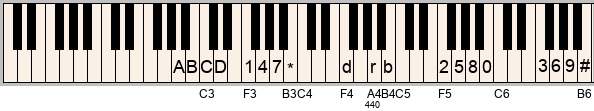
\includegraphics[scale=1.0]{demo/DTMF-layout.png}
   \caption{DTMF Layout on the Keyboard}
   \label{fig:cookbook_instruments_DTMF_layout}
\end{figure}

\subsection{Piano}
\label{subsec:cookbook_instruments_piano}

   TODO.

\subsection{Leads}
\label{subsec:cookbook_instruments_leads}

   TODO.

\subsection{Guitar}
\label{subsec:cookbook_instruments_guitar}

   \textsl{Yoshimi} ships with some mediocre acoustic and steel guitar
   patches, but some amazing distortion guitars.  We decided to try our hand
   at a 12-string guitar.

\subsubsection{Guitar / 12-String}
\label{subsubsec:cookbook_instruments_guitar_12_string}

   A 12-string guitar has pairs of strings, with each member of a pair an
   octave apart in frequency, for all strings but one.  We've provided two
   versions of an attempt at a 12-string.

   \index{guitar!12-string}
   The first 12-string simulation is stored in
   \index{files!12-string}
   \texttt{yoshimi/banks/demo/Low\_Octave\_12-String\_Guitar\_Harms.xiz}.

   This patch provides one voice only, but the \textbf{Voice Oscillator}
   provides the fundamental and two harmonics.  In this oscillator,
   \textbf{H.md} is set to \textbf{Pow}.
   \textbf{Base F.} is set to \textbf{Pulse}.
   Voice 1 also enables the \textbf{Filter Params} to get a more acoustic
   sound.  Still sounds a bit harpsichordy.  Probably both strings need to
   be more complex.

   The second 12-string simulation is stored in
   \index{files!12-string}
   \texttt{yoshimi/banks/demo/Unison\_12-String\_Guitar\_Harms.xiz}.
   This version is similar to the previous 12-string, but, in voice 1,
   \textbf{Unison} is enabled, and vibrator and phase randomness are added.
   This version sounds significantly richer.

\subsection{Strings} (individual and ensemble)
\label{subsec:cookbook_instruments_strings}

   TODO.

\subsection{Bass}
\label{subsec:cookbook_instruments_bass}

   TODO.

\subsection{Saxophones}
\label{subsec:cookbook_instruments_saxophones}

   TODO.

%-------------------------------------------------------------------------------
% vim: ts=3 sw=3 et ft=tex
%-------------------------------------------------------------------------------


% Banks and General MIDI

%-------------------------------------------------------------------------------
% cookbook_banks
%-------------------------------------------------------------------------------
%
% \file        cookbook_banks.tex
% \library     Documents
% \author      Chris Ahlstrom
% \date        2015-07-12
% \update      2015-07-15
% \version     $Revision$
% \license     $XPC_GPL_LICENSE$
%
%     Provides the cookbooks_banks section of yoshimi-cookbook.tex.
%
%-------------------------------------------------------------------------------

\section{Banks and General MIDI}
\label{sec:cookbook_banks}

   Banks are discussed quite heavily in the user manual \cite{yoshimidoc}.
   Banks have evolved quite a bit in \textsl{Yoshimi}, and are
   a powerful way to manage instruments, and more amenable to automation
   than ever.

   In this section, we will attempt to set up a basic bank that is
   compliant with the General MIDI specification.  In order to do so, we
   will cherry pick instruments from the package that is provided when
   \textsl{Yoshimi} is installed, renaming them as needed to fit into the
   appropriate General MIDI slot.

   One problem is the selection of the \textsl{best} instrument for a given
   General MIDI program number.  There are simply too many to be able to
   evaluate them all.

   For this recipe, the \texttt{banks} and \texttt{presets} directories will
   be stored in the following directory of this project:

   \begin{verbatim}
      yoshimi/gm/basic
   \end{verbatim}

\subsection{Creating a Basic GM Bank}
\label{subsec:cookbook_banks_basic_gm}

   Creating even a basic General MIDI bank is beset with issues, even if one
   has at hand a large number of pre-built instruments.

   First, what is the purpose of the General MIDI specific?  To provide a
   dependable set of instruments so that tunes will sound basically similar
   on different GM-compliant synthesizers.  That's about it.  It doesn't
   guarantee that the sounds are consistent, nor does it guarantee that they
   are all of high quality.  The "FX", "Lead", and "Pad" instruments provide
   ambiguous descriptions that a wide range of sounds might fit.
   Getting a complete and high-quality set of sounds is extremely difficult.

   Second, evaluating a large number of pre-built instruments takes a lot of
   work.  We'd done some of this work for another project, and never
   finished.  Nor is the naming of such instruments all that helpful; many
   of the file-names are misleading.  Finding decent matches for a GM
   instrument takes time.

   Third, there are many GM instruments for which we've been able to find no
   good \textsl{ZynAddSubFX}/\textsl{Yoshimi} counterpart.  The only options
   are to pick a tolerable match, build a tolerable match oneself, or just
   plug in any old sound and wait for others to step up.

   Nonetheless, let's forge ahead.  The project file
   \texttt{contrib/instrument.ods} is a \textsl{LibreOffice} spreadsheet
   that represents some research in finding GM-compatible instruments.
   It's pretty bad; maybe 50\% useful.

   We converted it to \texttt{contrib/gmcopy} to copy the files
   into the project directory \texttt{yoshimi/banks/gm/basic}.
   We show the banks in table~\ref{table:gm_basic_files}
   for convenience.

%-------------------------------------------------------------------------------
% gm_basic_table
%-------------------------------------------------------------------------------
%
% \file        gm_basic_table.tex
% \library     Documents
% \author      Chris Ahlstrom
% \date        2015-06-15
% \update      2015-07-18
% \version     $Revision$
% \license     $XPC\_GPL\_LICENSE$
%
%     Provides the concepts.
%
%-------------------------------------------------------------------------------

\label{table:gm_basic_files}
\begin{longtable}{|l l|}

\caption{GM Basic Files} \\

\hline
   \textbf{General MIDI Instrument} &
      \textbf{Yoshimi Instrument Used} \\
\hline
\endfirsthead

\hline
   \textbf{General MIDI Instrument} &
      \textbf{Yoshimi Instrument Used} \\
\hline
\endhead

\hline
   Continued next page & \\
\hline
\endfoot

\hline
   End of table & \\
\hline
\endlastfoot

   \textbf{0001-Acoustic Grand Piano} &
      SynthPiano/0033-Analog Piano 1 \\
   \textbf{0002-Bright Acoustic Piano} &
      SynthPiano/0034-Analog Piano 2 \\
   \textbf{0003-Electric Grand Piano} &
      SynthPiano/0143-Space Piano \\
   \textbf{0004-Honky-tonk Piano} &
      SynthPiano/0068-Synth Piano 3 fat \\
   \textbf{0005-Electric Piano 1} &
      Rhodes/0002-DX Rhodes 2 \\
   \textbf{0006-Electric Piano 2} &
      Rhodes/0007-Dig Rhodes \\
   \textbf{0007-Harpsichord} &
      olivers100/0026-Harpsichord \\
   \textbf{0008-Clavinet} &
      Misc Keys/0060-Clavinet 1 \\
   \textbf{0009-Celesta} &
      Bells/0002-Music\_Box \\
   \textbf{0010-Glockenspiel} &
      Bells/0011-Glass bells \\
   \textbf{0011-Music Box} &
      Bells/0013-Tiny bells \\
   \textbf{0012-Vibraphone} &
      Chromatic Percussion/0045-Vibes no\_trem \\
   \textbf{0013-Marimba} &
      Chromatic Percussion/0056-FM marimba \\
   \textbf{0014-Xylophone} &
      Will\_Godfrey\_Collection/0001-Xylophone \\
   \textbf{0015-Tubular Bells} &
      Chromatic Percussion/0097-Marimba 3 \\
   \textbf{0016-Dulcimer} &
      Plucked/0004-Plucked 4 \\
   \textbf{0017-Drawbar Organ} &
      Organ/0001-Organ 1 \\
   \textbf{0018-Percussive Organ} &
      Organ/0012-Organ 12 \\
   \textbf{0019-Rock Organ} &
      Organ/0068-Square Organ \\
   \textbf{0020-Church Organ} &
      Organ/0061-Great Organ \\
   \textbf{0021-Reed Organ} &
      Reed\_and\_Wind/0039-Reed 7 \\
   \textbf{0022-Accordion} &
      Organ/0097-Accordion Pad 1 \\
   \textbf{0023-Harmonica} &
      Reed\_and\_Wind/0099-Sharp Reed \\
   \textbf{0024-Tango Accordion} &
      Organ/0101-Accordion 1 \\
   \textbf{0025-Acoustic Guitar nylon} &
      Piano/0144-Soft Piano1 \\
   \textbf{0026-Acoustic Guitar steel} &
      Guitar/0065-Clean Guitar1 \\
   \textbf{0027-Electric Guitar jazz} &
      Guitar/0066-Electric Guitar \\
   \textbf{0028-Electric Guitar clean} &
      Guitar/0133-Smooth Guitar \\
   \textbf{0029-Electric Guitar muted} &
      Guitar/0035-Short \\
   \textbf{0030-Overdriven Guitar} &
      Guitar/0042-Trash Guitar 3 \\
   \textbf{0031-Distortion Guitar} &
      Guitar/0005-Dist Guitar 5 \\
   \textbf{0032-Guitar harmonics} &
      Laba170bank/0028-PianoBell \\
   \textbf{0033-Acoustic Bass} &
      Will\_Godfrey\_Collection/0045-Steel Bass \\
   \textbf{0034-Electric Bass finger} &
      Bass/0009-Electric bass 1 \\
   \textbf{0035-Electric Bass pick} &
      Bass/0041-Electric\_Bass \\
   \textbf{0036-Fretless Bass} &
      Bass/0050-Fretless Bass \\
   \textbf{0037-Slap Bass 1} &
      Rhodes/0042-Hard Rhodes1 \\
   \textbf{0038-Slap Bass 2} &
      olivers-100/0018-Bass Guitar - Slap \\
   \textbf{0039-Synth Bass 1} &
      Bass/0013-FM rubber bass \\
   \textbf{0040-Synth Bass 2} &
      Bass/0024-Moog bass \\
   \textbf{0041-Violin} &
      Strings/0051-Synth Violin 2 Fat \\
   \textbf{0042-Viola} &
      Strings/0051-Synth Violin 2 Fat \\
   \textbf{0043-Cello} &
      Strings/0051-Synth Violin 2 Fat \\
   \textbf{0044-Contrabass} &
      Bass/0005-Bass 5 \\
   \textbf{0045-Tremolo Strings} &
      Strings/0001-Saw Strings 1 \\
   \textbf{0046-Pizzicato Strings} &
      Strings/0003-Saw Strings 3 \\
   \textbf{0047-Orchestral Harp} &
      Pads/0065-Soft Pad \\
   \textbf{0048-Timpani} &
      Noises/0018-Gun \\
   \textbf{0049-String Ensemble 1} &
      VDX/0065-Strings \\
   \textbf{0050-String Ensemble 2} &
      folderol collection/0029-Full Strings \\
   \textbf{0051-Synth Strings 1} &
      Strings/0010-Strings Pad1 \\
   \textbf{0052-Synth Strings 2} &
      Strings/0014-Strings Pad5 \\
   \textbf{0053-Choir Aahs} &
      Choir\_and\_Voice/0001-AHH Choir 1 \\
   \textbf{0054-Voice Oohs} &
      Choir\_and\_Voice/0004-Voice OOH \\
   \textbf{0055-Synth Voice} &
      Choir\_and\_Voice/0005-Choir Pad1 \\
   \textbf{0056-Orchestra Hit} &
      Misc/0010-Industrial orchestra \\
   \textbf{0057-Trumpet} &
      Leads/0027-Prophet horn 2 \\
   \textbf{0058-Trombone} &
      Brass/0033-Analog Brass 1 \\
   \textbf{0059-Tuba} &
      Brass/0001-FM Thrumpet \\
   \textbf{0060-Muted Trumpet} &
      Synth/0001-Soft Synth 1 \\
   \textbf{0061-French Horn} &
      Brass/0034-Analog Brass 2 \\
   \textbf{0062-Brass Section} &
      Brass/0007-Synth Brass 5 \\
   \textbf{0063-Synth Brass 1} &
      Brass/0003-Synth Brazz 1 \\
   \textbf{0064-Synth Brass 2} &
      Brass/0004-Synth Brazz 2 \\
   \textbf{0065-Soprano Sax} &
      Reed\_and\_Wind/0066-Fat Reed2 \\
   \textbf{0066-Alto Sax} &
      Reed\_and\_Wind/0065-Fat Reed1 \\
   \textbf{0067-Tenor Sax} &
      Reed\_and\_Wind/0037-Reed 5 \\
   \textbf{0068-Baritone Sax} &
      Reed\_and\_Wind/0099-Sharp Reed \\
   \textbf{0069-Oboe} &
      Reed\_and\_Wind/0040-Reed 8 \\
   \textbf{0070-English Horn} &
      Brass/0034-Analog Brass 2 \\
   \textbf{0071-Bassoon} &
      Will\_Godfrey\_Collection/0102-Bassoon \\
   \textbf{0072-Clarinet} &
      Reed\_and\_Wind/0006-Clarinet \\
   \textbf{0073-Piccolo} &
      Will\_Godfrey\_Collection/0071-Ocarina \\
   \textbf{0074-Flute} &
      Will\_Godfrey\_Collection/0057-Soft Flute \\
   \textbf{0075-Recorder} &
      Will\_Godfrey\_Collection/0059-Ocarina \\
   \textbf{0076-Pan Flute} &
      Will\_Godfrey\_Collection/0127-Pan Pipe \\
   \textbf{0077-Blown Bottle} &
      Will\_Godfrey\_Collection/0125-Bottle \\
   \textbf{0078-Shakuhachi} &
      Will\_Godfrey\_Collection/0125-Pan Pipe 32 \\
   \textbf{0079-Whistle} &
      Will\_Godfrey\_Collection/0027-Ghost Whistle \\
   \textbf{0080-Ocarina} &
      Flute/0071-Ocarina \\
   \textbf{0081-Lead 1 square} &
      Leads/0022-Square lead \\
   \textbf{0082-Lead 2 sawtooth} &
      Louigi\_Verona\_Workshop/0008-saw-lead \\
   \textbf{0083-Lead 3 calliope} &
      Leads/0018-Sine lead \\
   \textbf{0084-Lead 4 chiff} &
      chip/0018-Chiffer\_Chip \\
   \textbf{0085-Lead 5 charang} &
      Louigi\_Verona\_Workshop/0001-progressive-lead-1 \\
   \textbf{0086-Lead 6 voice} &
      Choir\_and\_Voice/0067-Vocal Morph 3 \\
   \textbf{0087-Lead 7 fifths} &
      chip/0017-SuperSquare1 \\
   \textbf{0088-Lead 8 bass lead} &
      Strings/0157-Dual Strings Oct2 \\
   \textbf{0089-Pad 1 new age} &
      Pads/0028-Ethereal \\
   \textbf{0090-Pad 2 warm} &
      Will\_Godfrey\_Companion/0019-Warm Square Swell \\
   \textbf{0091-Pad 3 polysynth} &
      Dual/0065-Dream of the Saw \\
   \textbf{0092-Pad 4 choir} &
      Alex\_J/0100-Choir Pad \\
   \textbf{0093-Pad 5 bowed} &
      The\_Mysterious\_Bank/0004-trance\_strings\_pad \\
   \textbf{0094-Pad 6 metallic} &
      The\_Mysterious\_Bank/0011-dreaming\_bells \\
   \textbf{0095-Pad 7 halo} &
      Alex\_J/RadioPulsePad \\
   \textbf{0096-Pad 8 sweep} &
      Pads/0011-lightbeam \\
   \textbf{0097-FX 1 rain} &
      The\_Mysterious\_Bank/0037-the\_rain \\
   \textbf{0098-FX 2 soundtrack} &
      The\_Mysterious\_Bank/0038-falling\_stars \\
   \textbf{0099-FX 3 crystal} &
      Will\_Godfrey\_Companion/0006-Tinkle Bell \\
   \textbf{0100-FX 4 atmosphere} &
      The\_Mysterious\_Bank/0038-the\_starting\_machine \\
   \textbf{0101-FX 5 brightness} &
      Noises/0014-droplets for chords \\
   \textbf{0102-FX 6 goblins} &
      Noises/0002-Ioioioioioi \\
   \textbf{0103-FX 7 echoes} &
      Noises/0072-Cave Gates \\
   \textbf{0104-FX 8 sci-fi} &
      The\_Mysterious\_Bank/0031-etrange\_sound \\
   \textbf{0105-Sitar} &
      olivers-100/0019-FM Sitar \\
   \textbf{0106-Banjo} &
      olivers-100/0016-Banjoey \\
   \textbf{0107-Shamisen} &
      Plucked/0034-Plucked String2 \\
   \textbf{0108-Koto} &
      Plucked/0003-Plucked 3 \\
   \textbf{0109-Kalimba} &
      Plucked/0001-Plucked 1 \\
   \textbf{0110-Bagpipe} &
      Reed\_and\_Wind/0033-Reed 1 \\
   \textbf{0111-Fiddle} &
      Laba170bank/0055-DevilsFiddle2 \\
   \textbf{0112-Shanai} &
      Reed\_and\_Wind/0035-Reed 3 \\
   \textbf{0113-Tinkle Bell} &
      Bells/0011-Glass bells \\
   \textbf{0114-Agogo} &
      The\_Mysterious\_Bank/0028-snare \\
   \textbf{0115-Steel Drums} &
%     C\_Ahlstrom/Add\_Pseudo\_Steel\_Drums\_2 \\   Found one even better!
      olivers-100/0029-Steel Drums \\
   \textbf{0116-Woodblock} &
      The\_Mysterious\_Bank/0028-snare \\
   \textbf{0117-Taiko Drum} &
      The\_Mysterious\_Bank/0028-snare \\
   \textbf{0118-Melodic Tom} &
      demo/Melodic\_Tom\_from\_Nat\_drum\_kit \\
   \textbf{0119-Synth Drum} &
      The\_Mysterious\_Bank/0028-snare \\
   \textbf{0120-Reverse Cymbal} &
      The\_Mysterious\_Bank/0028-snare \\
   \textbf{0121-Guitar Fret Noise} &
      The\_Mysterious\_Bank/0028-snare \\
   \textbf{0122-Breath Noise} &
      The\_Mysterious\_Bank/0028-snare \\
   \textbf{0123-Seashore} &
      Noises/0008-Wind and Surf \\
   \textbf{0124-Bird Tweet} &
      The\_Mysterious\_Bank/0028-snare \\
   \textbf{0125-Telephone Ring} &
      The\_Mysterious\_Bank/0028-snare \\
   \textbf{0126-Helicopter} &
      The\_Mysterious\_Bank/0028-snare \\
   \textbf{0127-Applause} &
      The\_Mysterious\_Bank/0028-snare \\
   \textbf{0128-Gunshot} &
      Noises/0018-Gun \\
   \textbf{0129-Drum Kit} &
      C\_Ahlstrom/Natural\_Drum\_Kit\_Basic \\
\end{longtable}

%-------------------------------------------------------------------------------
% vim: ts=3 sw=3 et ft=tex
%-------------------------------------------------------------------------------


   Presumably, this basic bank could be improved enough to be useful
   for most music.  Alternative (and better) banks could be created, as
   well.

\subsection{Root Paths}
\label{subsec:cookbook_banks_root_paths}

   The first thing to do is to add the yoshimi-cookbook banks directory to 
   your setup.

   Run \textsl{Yoshimi}, and navigate the following user-interface path:
   \textsl{Menu / Instrument / Show Root Paths ...}

   Then click \textbf{Add root directory...}.  Navigate to where the
   yoshimi-cookbook project is stored and add the \texttt{yoshimi/banks}
   directory.  The result should be something like the following:

\begin{figure}[H]
   \centering 
   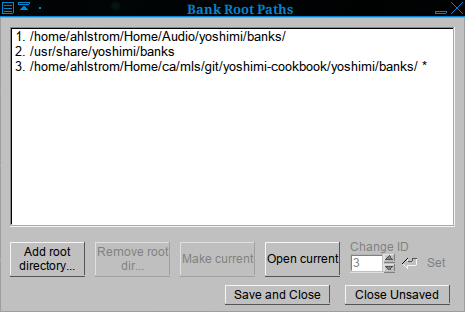
\includegraphics[scale=1.0]{menu/Instrument/bank_root_paths.png}
   \caption{Bank Root Paths}
   \label{fig:cookbook_bank_root_paths}
\end{figure}

   Click on the new directory.
   It has ID = 2 in that diagram.  We will refer to this value as
   the "GM path ID", and the actual path as the "GM path".
   Now click the \textbf{Make current} button.
   Verify that it now has the asterisk. 
   Click the \textbf{Save and Close} button.

   Now let's open the "gm-basic" bank.
   Run \textsl{Yoshimi}, and navigate the following user-interface path:
   \textsl{Menu / Instrument / Show Banks ...}

   In the matrix of banks, you should see "gm-basic" somewhere.
   (We also have a "demo" bank in place.)

\begin{figure}[H]
   \centering 
   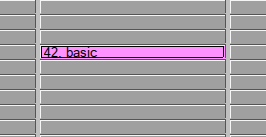
\includegraphics[scale=1.0]{menu/Instrument/solitary_basic_bank.png}
   \caption{One Basic Bank}
   \label{fig:cookbook_bank_solitary_bank}
\end{figure}
   
   Click on the "gm-basic" bank.  The larger dialog below will be shown.

\begin{figure}[H]
   \centering 
   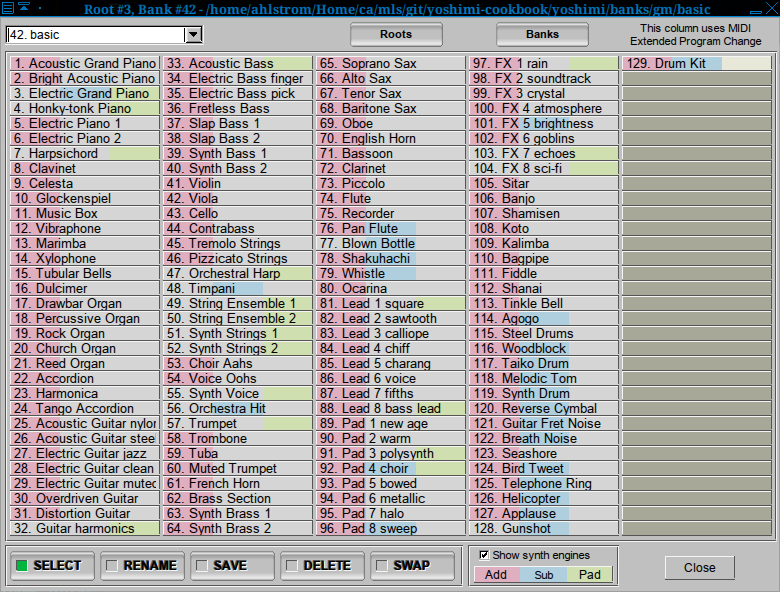
\includegraphics[scale=1.0]{menu/Instrument/banks_gm_basic.png}
   \caption{A General MIDI Basic Bank}
   \label{fig:cookbook_bank_basic_bank}
\end{figure}

Remember that these banks have GM names; the original files used to create
each one are listed in the spreadsheet mentioned in the previous section.

Also note the drum kit, with an ID of 129.  Normally, drum kits might be
stored in a bank of drum kits, but here we have a GM-compliant drum kit,
compliant in the sense that most of the keys are mapped correctly,
and all keys will play \textsl{something}.

%-------------------------------------------------------------------------------
% vim: ts=3 sw=3 et ft=tex
%-------------------------------------------------------------------------------


% %-------------------------------------------------------------------------------
% cookbook_concepts
%-------------------------------------------------------------------------------
%
% \file        cookbook_concepts.tex
% \library     Documents
% \author      Chris Ahlstrom
% \date        2015-07-15
% \update      2015-07-16
% \version     $Revision$
% \license     $XPC_GPL_LICENSE$
%
%     Provides the concepts.
%
%-------------------------------------------------------------------------------

\section{Concepts}
\label{sec:concepts}

   This section, like its counterpart in our \textsl{Yoshimi User Manual},
   presents some useful concepts, while keeping them out of the way.

\subsection{Concepts / Terms}
\label{subsec:concepts_terms}

   This section doesn't provide comprehensive coverage of terms.  It
   covers mainly terms that puzzled the author at first or that are
   necessary to understand the recipes.

\subsubsection{Concepts / Terms / cent}
\label{subsubsec:concepts_terms_cent}

   The \textbf{cent}
   \index{cent}
   is a logarithmic unit of measure used for musical
   intervals.  Twelve-tone equal temperament divides the octave into 12
   semitones of 100 cents each. Typically, cents are used to measure
   extremely small finite intervals, or to compare the sizes of comparable
   intervals in different tuning systems.
   The interval of one cent is much too small to be heard between
   successive notes.

   Since the detuning provided in \textsl{Yoshimi} is based primarily on
   cents (and octaves), it pays to understand cents.  If a given frequency
   \texttt{f'} is offset from another frequency \texttt{f}, the
   relationships between them in semitones are:

   \[f' = f * 2^s/12\]

   \[s = 12 log (f'/f) / log 2\]

   In cents, these relationships become:

   \[f' = f * 2^s/1200\]

   \[s = 1200 log (f'/f) / log 2\]

   These relationships hold whether \texttt{f'} is less than or greater than
   \texttt{f}.  They provide an easy way to determine how much to detune a
   frequency in \textsl{Yoshimi}.

\subsubsection{Concepts / Terms / ring modulation}
\label{subsubsec:concepts_terms_ring_mod}

   \textbf{Ring modulation}
   \index{ring modulation}
   \index{modulation!ring}
   is the multiplication (heterodyning) of two signals, and is named for the
   ring-like circuit that can produce it.
   When two tones, \texttt{f1} and \texttt{f2}, with 
   \texttt{f1} \textless \texttt{f2}, are multiplied, the spectrum
   changes from \{f1, f2\} to \{f2-f1, f2+f1\}.

   Depending on the ratio of \texttt{f1} and \texttt{f2}, the
   sounds can be bell-like or very discordant.
   \textsl{Yoshimi} provides ring modulation, as well as other forms of
   modulation.

%-------------------------------------------------------------------------------
% vim: ts=3 sw=3 et ft=tex
%-------------------------------------------------------------------------------


\section{Summary}
\label{sec:summary}

   In summary, we can say that you will absolutely love 
   cooking with \textsl{Yoshimi}.

% References

%-------------------------------------------------------------------------------
% cookbook_references
%-------------------------------------------------------------------------------
%
% \file        cookbook_references.tex
% \library     Documents
% \author      Chris Ahlstrom
% \date        2015-07-12
% \update      2015-07-15
% \version     $Revision$
% \license     $XPC_GPL_LICENSE$
%
%     Provides the References section of yoshimi-cookbook.tex.  Rather
%     than use the bibtex package, our small set of references uses a
%     simpler method.
%
%-------------------------------------------------------------------------------

\section{References}
\label{sec:cookbook_references}

   The \textsl{Yoshimi} cookbook reference list.

\begin{thebibliography}{99}

   \bibitem{bankrootupgrades}
   Will J. Godfrey
   \emph{A discussion of making Bank/Root specifications more regular.}
   \url{http://sourceforge.net/p/yoshimi/mailman/message/33200765/}
   2014.

   \bibitem{bellsimple}
   Blair School of Music, Vanderbilt University.
   \emph{Creating a Simple Bell}
   \url{http://computermusicresource.com/Simple.bell.tutorial.html}
   2012?

   \bibitem{bellspectrum}
   FM 8 Tutorials
   \emph{Spectrum of a Simple Bell}
   \url{http://www.fm8tutorials.com/wp-content/uploads/2012/03/Bell-spectrum.png}
   2012?

   \bibitem{ringmodulator}
   LinuxMusicians newsgroup
   \emph{Ring Modulation in ZynAddSubFX}
   \url{http://linuxmusicians.com/viewtopic.php?f=1&t=8178}
   2012.

   \bibitem{scala}
   Manuel Op de Coul <\url{coul@huygens-fokker.org}>
   \emph{The Scala Musical Tuning Application.}
   \url{http://www.huygens-fokker.org/scala/}
   Scala is a powerful software tool for experimentation with musical
   tunings, such as just intonation scales, equal and historical
   temperaments, microtonal and macrotonal scales, and non-Western scales.
   2014.

   \bibitem{sharphall}
   Sharphall
   \emph{How to create drum sounds in ZynAddSubFX or Yoshimi, Part 1}
   \url{http://sharphall.org/docs/zynaddsubfx\_yoshimi\_drum\_tutorial.php}
   Never got continued, unfortunately.

   \bibitem{synthsecrets}
   Gordon Reid
   \emph{Synth Secrets:  Creative Synthesis}
   \url{http://www.soundonsound.com/sos/allsynthsecrets.htm}
   1999-2004.

   \bibitem{yoshimi}
   Yoshimi team \url{abrolag@users.sourceforge.net}
   \emph{The download site for the Yoshimi software synthesizer.}
   \url{http://yoshimi.sourceforge.net/}
   2015.

   \bibitem{yoshimi2}
   Yoshimi team
   \emph{The alternate location for the Yoshimi source-code.}
   \url{https://github.com/abrolag/yoshimi/}
   2015.

   \bibitem{yoshimidoc}
   Chris Ahlstrom
   \emph{A Yoshimi User Manual.}
   \url{https://github.com/ahlstromcj/yoshimi-doc/}
   2015.
   

\end{thebibliography}

%-------------------------------------------------------------------------------
% vim: ts=3 sw=3 et ft=tex
%-------------------------------------------------------------------------------


\printindex

\end{document}

%-------------------------------------------------------------------------------
% vim: ts=3 sw=3 et ft=tex
%-------------------------------------------------------------------------------
